\documentclass{winnower}
\usepackage{indentfirst}
\usepackage{graphicx}
\usepackage{caption}
\usepackage{tocbibind}
\usepackage{subfigure}
\usepackage{xcolor}
\usepackage{float}
\usepackage[section]{placeins}
\usepackage{multirow}
\usepackage{booktabs}
\setlength{\belowcaptionskip}{-0.5cm}

\begin{document}

\title{Black-Litterman Portfolios with Machine Learning derived Views}

\author{Haoyu Guan}
\author{Yishuang Bao}
\author{Ruizhe He}
\author{Ziqi Chen}
\author{Yifei Zhang}
\affil[1]{Questrom School of Business, Boston University}







\date{2019.12.11}

\maketitle

\begin{abstract}
In this report, we build various Black-Litterman models on a multi ETF portfolio and test their performance.
Following Meucci(2010)[1], we build our own set of view matrix $Q_t$ and $P$ using Machine Learning classifiers to calculate conditional expected return. And we also do the back testing process to evaluate the performance of the whole model.
\end{abstract}


%-------------------------------------------------%
\section{Introduction}
%-------------------------------------------------%


\indent At a time when portfolio optimization used to take as inputs only the expectations and the covariances of a set of assets computed from a given reference model. The Black-Litterman asset allocation model , created by Black and Litterman put view portfolios,the expected returns on those portfolios,the confidence in the view portfolios and the uncertainty on the reference model.

It is an asset allocation model which has its roots in mean-variance optimization model and capital asset pricing model (CAPM). Model builds on mean variance optimization and CAPM by using a Bayesian framework that allows investors to incorporate their views on markets
effectively into asset allocation process. Main contribution of Black-Litterman model is that, it enables investors to construct sensible portfolios without using unnecessary constraints which also reflect their views on markets.

It is well known to both academics and practitioners that standard mean variance optimization is very sensitive to expected returns and often generates extreme portfolios (concentration in very few assets, large long and short positions). Black-Litterman model overcomes these issues by choosing a neutral reference point, CAPM equilibrium. It also allows investors to express their views with varying confidence levels and integrate these views into CAPM prior by using a Bayesian framework

\section{Data}
To construct multi-asset portfolios we include highly liquid ETFs which have a wide coverage of
the broader asset classes and constitute a globally diversified multi-asset portfolio, representing
MSCI-EAFE and MSCI-Emerging markets, U.S. Treasuries (long term), Gold bullion and the
U.S. real estate sector. We use the iShares MSCI EAFE ETF (EFA) which tracks MSCI EAFE
index, and iShares MSCI Emerging Markets ETF (EEM) which tracks an index composed
of large and mid cap emerging markets to cover both developed and emerging markets. Also we use SPDR Gold Shares (GLD) to represent the gold market, and iShares US
Real Estate ETF (IYR) to represent the US Real Estate Market.

\begin{figure*}[h]
\begin{center}
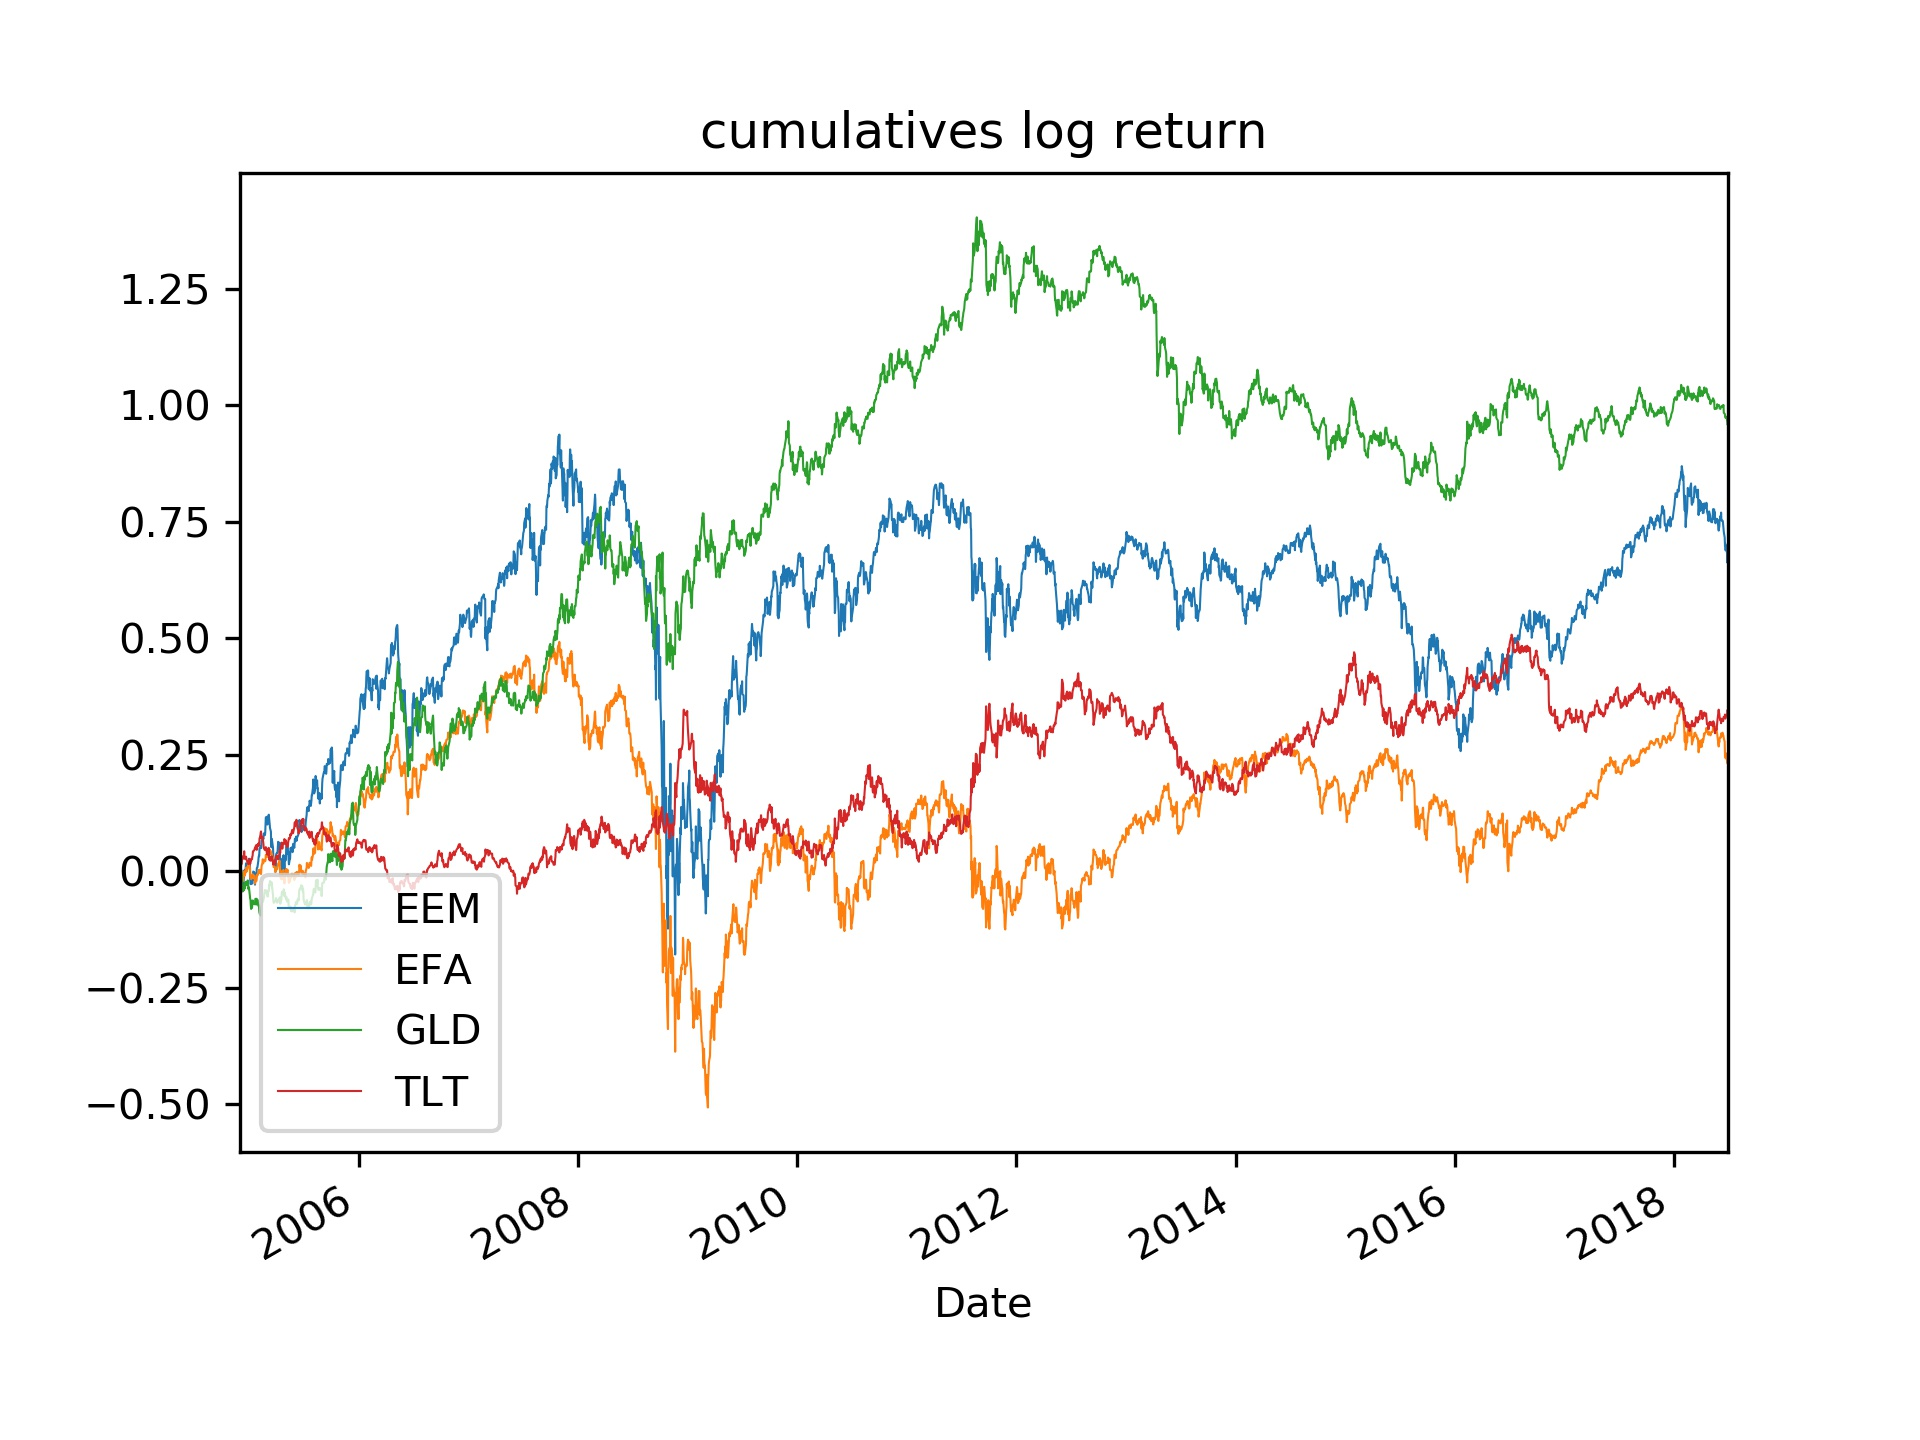
\includegraphics[scale=0.7]{1_2.jpg}
\caption
{Cumulative excess return of the assets for the period June 2005 - Dec. 2019}
\label{fig:f1}
\end{center}
\end{figure*}

The ETFs selected for this study are relatively recent but have continuous daily pricing
history available since June 2005. We obtain weekly data for the period from December
2005 to December 2019 from Yahoo Finance. This period includes one full bear market (2007-2009)
and two bull markets (2005-2007 and 2009-May 2013), thus insulating the study from explicit
market-phase bias. All data are denominated in US dollar. The Market Capitalization of these
ETFs are obtained from ETF Database.
\section{Methodology}

\begin{figure*}[h]
\begin{center}
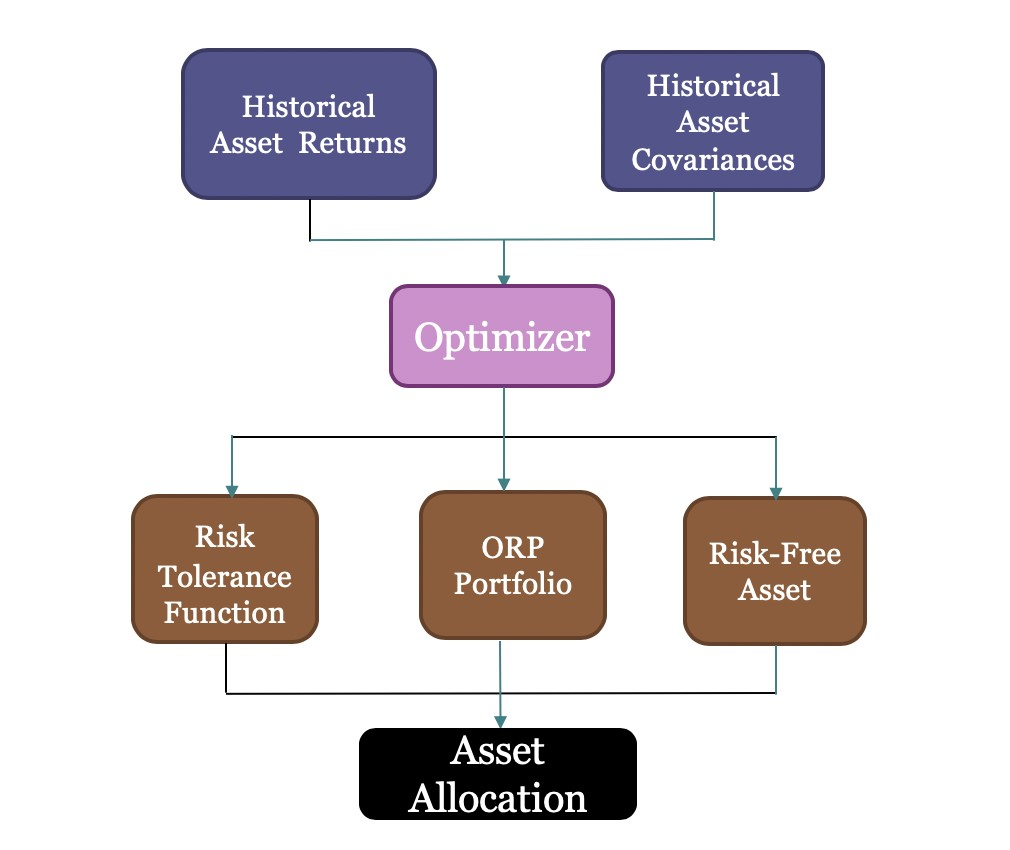
\includegraphics[scale=0.55]{1_1.jpg}
\caption
{Mean-Variance optimization process}
\label{fig:f1}
\end{center}
\end{figure*}


\begin{figure*}[!h]
\begin{center}
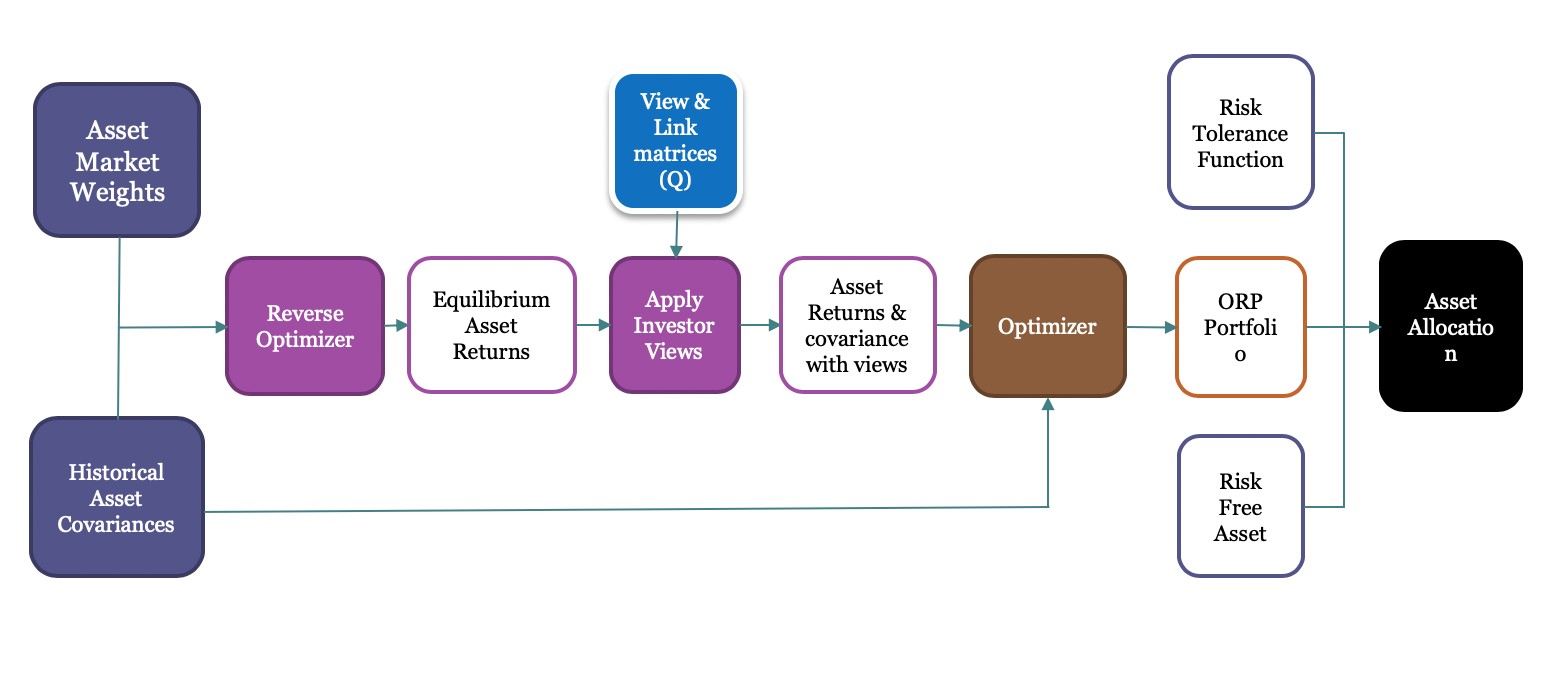
\includegraphics[scale=0.45]{1_3.jpg}
\caption
{Black-Litterman optimization process}
\label{fig:f1}
\end{center}
\end{figure*}

\subsection{Reverse Optimization}
Instead of using the historical asset return, BL use the equilibrium asset returns. Equilibrium asset returns are returns implied from the market capitalization weights of individual assets or asset classes. It can be derived by a reverse optimization method in which the vector of implied excess equilibrium using the formula:

$$\Pi=\lambda\Sigma\omega_{mkt}$$

\noindent
where\\
$\Pi$ is the Implied Excess Equilibrium Return Vector (N x 1 column vector);\\
$\lambda$ is the risk aversion coefficient;\\
$\Sigma$ is the covariance matrix of excess returns (N x N matrix);\\
$\omega_{mkt}$ is the market capitalization weight (N x 1 column vector) of the assets.

\subsection{Black-Litterman Model}
\subsubsection{The Black-Litterman Formula}
The formula for the new Combined Return Vector ($E[R]$)
$$E[R]=[(\tau\Sigma)^{-1}+P^{'}\Omega^{-1}P]^{-1}[(\tau\Sigma)^{-1}\Pi+P^{'}\Omega^{-1}Q]$$

\noindent
Where\\
$\tau$ is a scalar;\\
$Q$ is the View Vector (k x 1 column vector)\\
$\Sigma$ is the covariance matrix of excess returns (N x N matrix);\\
$P$ is a matrix that identifies the assets involved in the views;\\
$\Pi$ is the Implied Equilibrium Return Vector (N x 1 column vector);\\
E[R] is the new(posterior) Combined Return Vector (N x 1 column vector);\\
$\Omega$ is a diagonal covariance matrix of error terms from the expressed views representing the uncertainty in each view (K x K matrix);

\subsubsection{Calculating the New Combined Return Vector}
Our focus in the estimation is the combination of conditional equilibrium returns with the views using Bayesian approach. The process of combining the subjective views of an investor regarding to the expected returns of one or more assets with the market equilibrium vector of expected return is described in the Figure 3.

\begin{figure*}[h]
\begin{center}
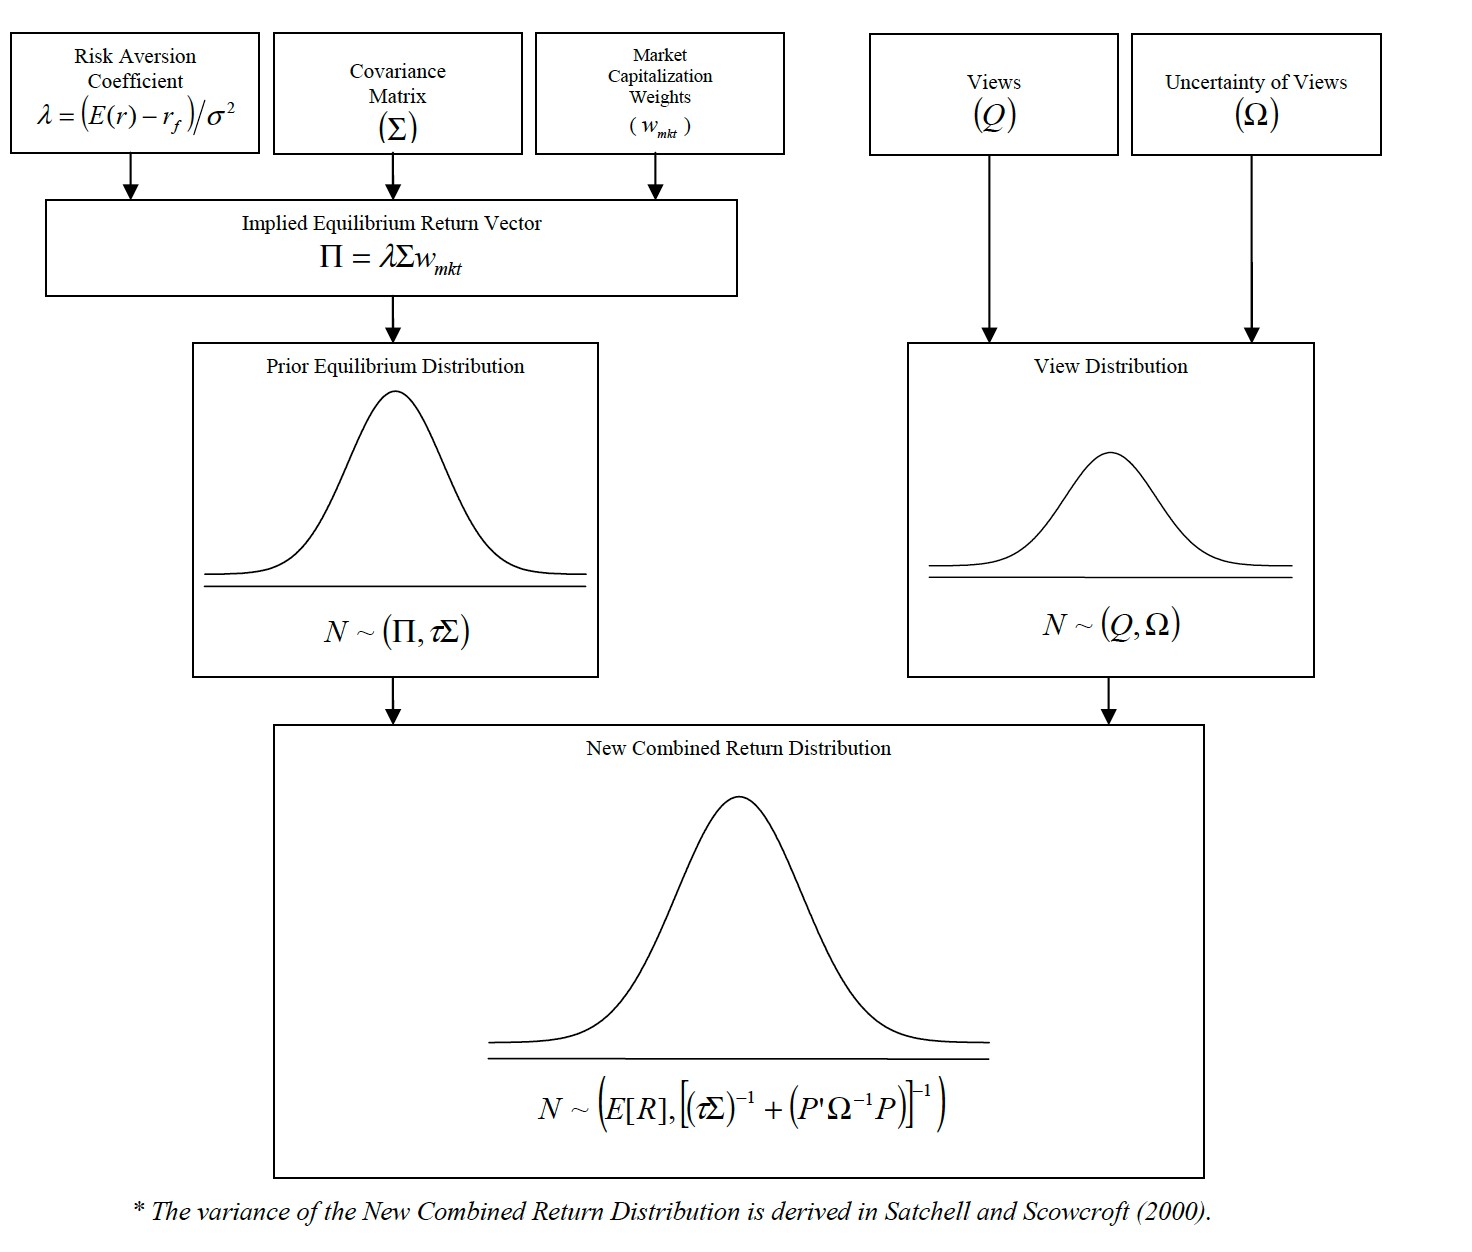
\includegraphics[scale=0.55]{1_4.jpg}
\caption
{Deriving the New Combined Return Vector (E[R])}
\label{fig:f1}
\end{center}
\end{figure*}

\subsection{Risk Adjusted Black-Litterman Portfolios}
We discussed the reversed optimizer above and following is the discussion of the forward optimizer.

\subsubsection{Sharp Ratio Maximazation}
In the method we use mean variance optimization and maximize the Sharpe ratio.
$$\max{\dfrac{\omega^{'}_{BL,t}\mu_{BL,t}}{\sqrt{\omega^{'}_{BL,t}\Sigma_{BL,t}\omega_{BL,t}}}}$$
where
$$\omega^{'}_{BL,t}\textbf{1}=1$$

\noindent
Where\\
$\mu_(BL,t)$ is the expected excess return of the BL portfolio $E[R]$\\
$\omega_(BL,t)^{'}\Sigma\omega_(BL,t)$ is the conditional portfolio variance\\
$\omega_(BL,t)$ is the N x 1 vector of portfolio weights

Thus, the vector of optimal weights for the SR-BL portfolio is given by
$$\omega^{*}_{BL,t}=\dfrac{\Sigma^{-1}_{BL,t}\mu_{BL,t}}{\textbf{1}^{'}\Sigma^{-1}_{BL,t}\mu_{BL,t}}$$

From 2.2.2 the individual variances of the error term $(\omega)$ that form the diagonal elements of the covariance matrix of the error term $(\Omega)$ were based on the variances of the view portfolios ($p_k\Sigma p_k$) multiplied by the scalar($\tau$). However, it is my opinion that  there may be other sources of information in addition  to the variance of the view portfolio that affect an investor��s confidence  in a view.

Setting all of the diagonal elements of $\Omega$ equal to zero is equivalent to specifying $100\%$ confidence in all of the K views. When $100\%$ confidence is specified for all of  the views, the Black-Litterman formula for the New Combined Return Vector under $100\%$ certainty$(E[R_{100\%}])$ is
$$E[R_{100\%}]=\Pi+\tau\Sigma P^{'}(P\tau\Sigma P^{'})^{-1}(Q-P\Pi)$$

Substituting $E([R_{100\%}])$ for $E[R]$ leads to $w_{100\%}$, the weight vector based on $100\%$ confidence in the views. $w_{100\%}, w_{mkt}$ and $w_{bl}$.

To determine the implied level of confidence in the views, we divide each weight difference$(w_{bl} - w_{mkt})$ by the corresponding maximum weight difference$(w_{100\%} - w_{mkt})$. The confidence levels are about $43\%$.





\section{Machine Learning}
\subsection{Label Generation}

As mentioned before, we need a $Q$ matrix for each period as the input of our Black-Litterman model. By transformation, the equation of $Q$ is:

\begin{equation}
Q_t(k)=(P_t \pi_t)(k)+\eta_k\sqrt{(P_t \sigma_t P_t^{'})(k,k)} \quad\quad k=1,2,...,K
\label{Qeta}
\end{equation}

We are going to apply machine learning methods on $\eta$ above. For each period $t$, we will generate a vector of $\eta$, and $k$ here is the $k$-th view. We use rolling classifier (150 previous data) to fit a model and use it to predict next week's $\eta$.

To use machine learning, we need to first generate our label. Here we define $\eta$ into 4 classes: $\eta\in\{-2,-1,1,2\}$, which is "Very Bearish", "Bearish", "Bullish" and "Very Bullish" respectively. We now need two classifiers to classify them. The first one $Y_1$ is the sign and the second one $Y_2$ is absolute value. The definition is as below:

\begin{equation}
Y_1=\left\{
	\begin{aligned}
	&-1, \text{if sign of excess return of next week's is negative} \\
	&+1, \text{if sign of excess return of next week's is positive} \\
	\end{aligned}
\right.
\label{y1}
\end{equation}

\begin{equation}
Y_2=\left\{
	\begin{aligned}
	&1, \text{if }z_t=\frac{r_t-\bar{r}_{t,3}}{\sigma_{t,3}}\leq 1\\
	&2, \text{if }z_t=\frac{r_t-\bar{r}_{t,3}}{\sigma_{t,3}}>1 \\
	\end{aligned}
\right.
\label{y2}
\end{equation}

Finally, we multiply $Y_1$ and $Y_2$ to generate the final label of $\eta$.

\subsection{Feature Generation}

Feature is very important for machine learning. Good features will help to fit model with better performance. Here we choose different kinds of indicators to consider different aspects that influence the performance of the ETFs. Different features are chosen as follows:

\begin{enumerate}

\item[$\bullet$] Returns and excess returns of 4 ETFs and S$\&$P 500, VIX, and 10 Year treasury note yield index.

\item[$\bullet$] Rate of change of volume of 4 ETFs.

\item[$\bullet$] Momentum indicators: CCI, RSI and Fast Stochastic Oscillator of 4 ETFs and S$\&$P 500, VIX, and 10 Year treasury note yield index.

\item[$\bullet$] Trend indicators: SMA, EMA and MACD of 4 ETFs and S$\&$P 500, VIX, and 10 Year treasury note yield index.

\item[$\bullet$] Volatility indicators: Bollinger Bands and Volatility Ratio of 4 ETFs and S$\&$P 500, VIX, and 10 Year treasury note yield index.

\end{enumerate}

We put the indicators of different ETF's together to consider the correlation between those ETF's. We also calculated previous 1-4 weeks' period of indicators and their 1-3 lags to consider time series issue. Eventually, we generate 1324 different features.

\subsection{Feature Selection}

After generating those 1324 features, we want to select the important features and use them to fit our machine learning model to avoid overfitting. For each ETF's 2 different classifiers, we will process a feature selection. We select 10 most important features and therefore we will generate 8 feature matrices.

While processing feature selection, we use the Extra Tree Classifier. Extra Tree Classifier is a version of Random Forest. It is a kind of ensemble learning algorithms which gathers the result of multiple independent decision trees and combine them into the output of feature ranking. The difference between Extra Tree Classifier and Random Forest is that when splitting the nodes, Random Forest select the best feature based on some criteria, such as information gain and Gini Index, but Extra Tree Classifier select the beat feature randomly. Therefore, Extra Tree Classifier has better generalization probability than Random Forest. This is why we choose it to be our feature selection method.

When label generation and feature selection is finished, we can move forward to train our machine learning model and give out the prediction of $\eta$.

\subsection{Classification}

The process of applying supervised machine learning to a real-world problem is described in Figure 1. The data processing part and feature selection part is mention are mentioned above. The crucial part for machine learning classifications is algorithm selection. There are many supervised classifiers. In this article, we will use some typical classifiers as well as some modern ensemble learning classifiers:

\begin{figure*}[h]
\begin{center}
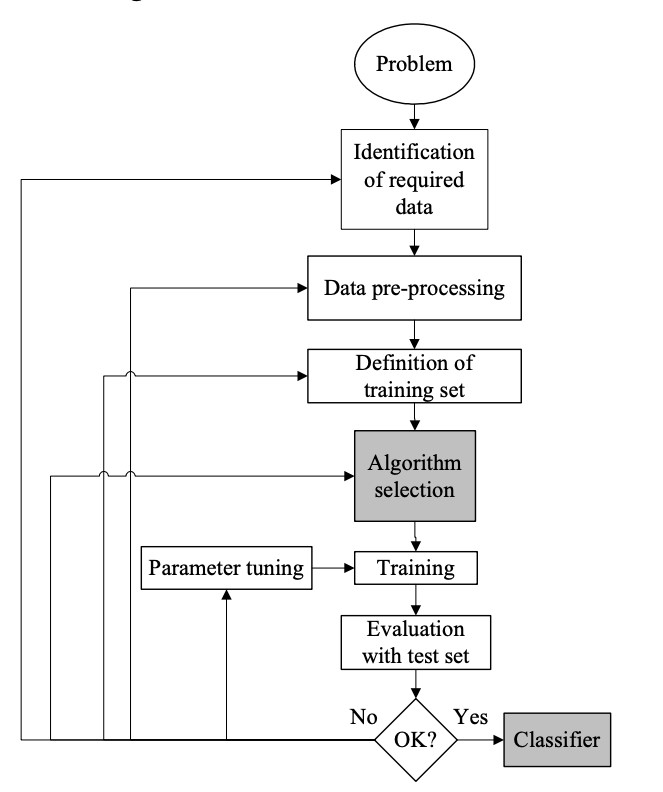
\includegraphics[scale=0.55]{1_5.jpg}
\caption
{Classification}
\label{fig:f1}
\end{center}
\end{figure*}


\begin{enumerate}

\item[$\bullet$]Logistic Regression:
Logistic regression is a classification algorithm used to assign observations to a discrete set of classes. Instead of fitting a straight line or hyperplane, the logistic regression model uses the logistic function to squeeze the output of a linear equation between 0 and 1.
\item[$\bullet$]Support Vector Machine:
Support vector machine (SVM) is a discriminative classifier formally defined by a separation hyperplane. That is, given labeled training data, SVM will output the optimal hyperplane that classifies the new instances. SVM can also perform a non-linear classification using kernel trick.
\item[$\bullet$]Naive Bayes:
The Naive Bayes Classifier technique is based on the Bayesian theorem and is particularly suited when the dimensionality of the inputs is high.


\item[$\bullet$]Ensemble methods: Ensemble methods
Ensemble methods are meta-algorithms that combine several machine learning techniques into one predictive model in order to decrease variance (bagging), bias (boosting), or improve predictions (stacking). In this article we will use AdaBoost, Gradient Boosting and Random Forest algorithms.

\end{enumerate}

Then we will build classifiers for each ETF and class (y1 or y2). We say that training a classifier is actually finding suitable parameters for the supervised learning algorithm, which makes it perform best in the test set. We use AUC-ROC curve (Area Under the Receiver Operating Characteristics curve) as our evaluation metrics. It is a performance measurement for classification problem at various thresholds settings. Based on this evaluation metrics, we use cross-validation grid search to find the optimal parameters.

Below are AUC-ROC curves of each classifier for each ETF��s y1 and y2. For convenience, the time period of training set we use here is the whole time period, while actually we use a rolling window basis.


\begin{figure}[!h]
\centering
\subfigure[EEM1]{
\begin{minipage}[h]{0.5\linewidth}
\centering
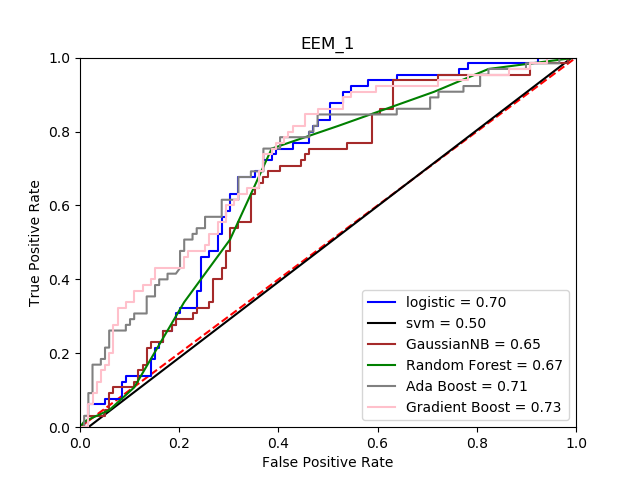
\includegraphics[width=2in]{EEM_1.png}
%\caption{fig1}
\end{minipage}%
}%
\subfigure[EEM2]{
\begin{minipage}[h]{0.5\linewidth}
\centering
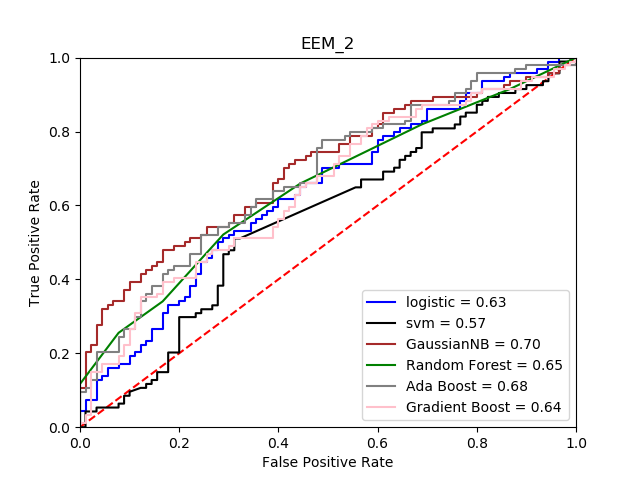
\includegraphics[width=2in]{EEM_2.png}
%\caption{fig2}
\end{minipage}%
}%
\centering
\caption{ROC curves related to EEM}
\end{figure}

\begin{figure}[!h]
\centering
\subfigure[EFA1]{
\begin{minipage}[h]{0.5\linewidth}
\centering
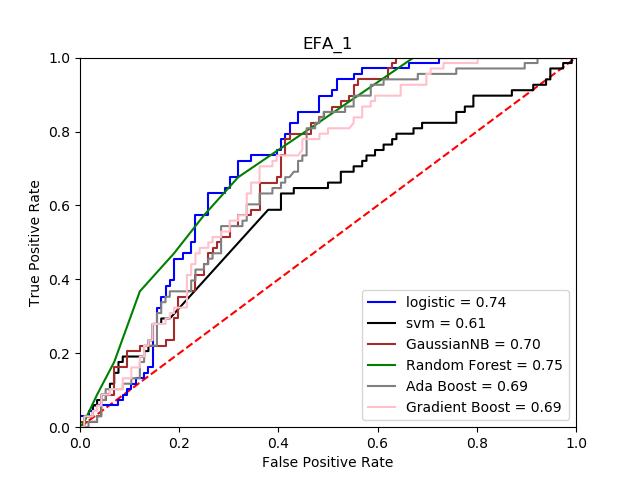
\includegraphics[width=2in]{EFA_1.png}
%\caption{fig1}
\end{minipage}%
}%
\subfigure[EFA2]{
\begin{minipage}[h]{0.5\linewidth}
\centering
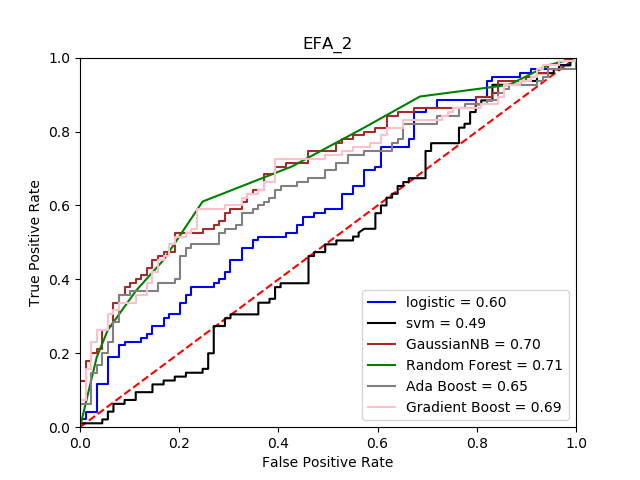
\includegraphics[width=2in]{EFA_2.png}
%\caption{fig2}
\end{minipage}%
}%
\centering
\caption{ROC curves related to EFA}
\end{figure}

\begin{figure}[!h]
\subfigure[GLD1]{
\begin{minipage}[h]{0.5\linewidth}
\centering
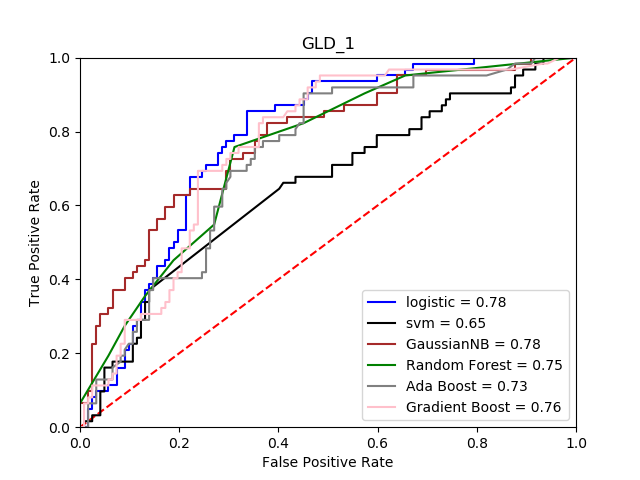
\includegraphics[width=2in]{GLD_1.png}
%\caption{fig1}
\end{minipage}%
}%
\subfigure[GLD2]{
\begin{minipage}[h]{0.5\linewidth}
\centering
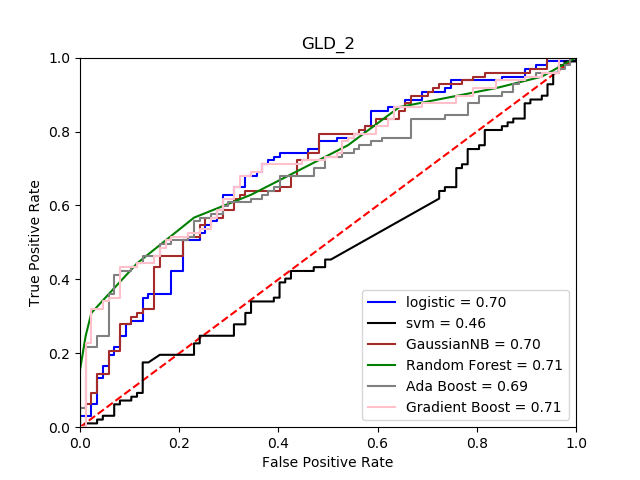
\includegraphics[width=2in]{GLD_2.png}
%\caption{fig2}
\end{minipage}%
}%
\caption{ROC curves related to GLD}
\end{figure}

\begin{figure}[!h]
\subfigure[IYR1]{
\begin{minipage}[h]{0.5\linewidth}
\centering
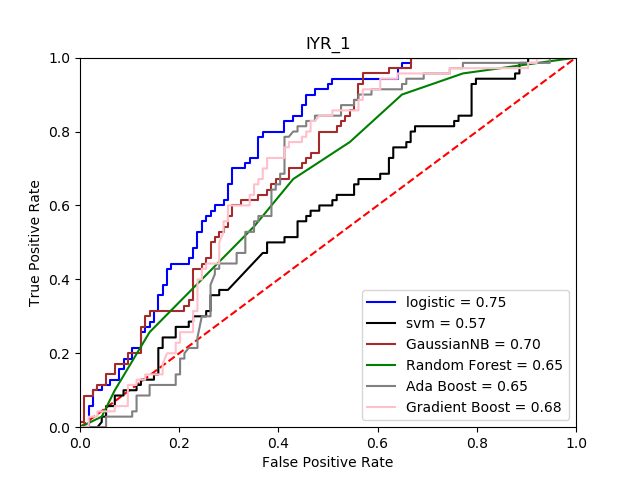
\includegraphics[width=2in]{IYR_1.png}
%\caption{fig1}
\end{minipage}%
}%
\subfigure[IYR2]{
\begin{minipage}[h]{0.5\linewidth}
\centering
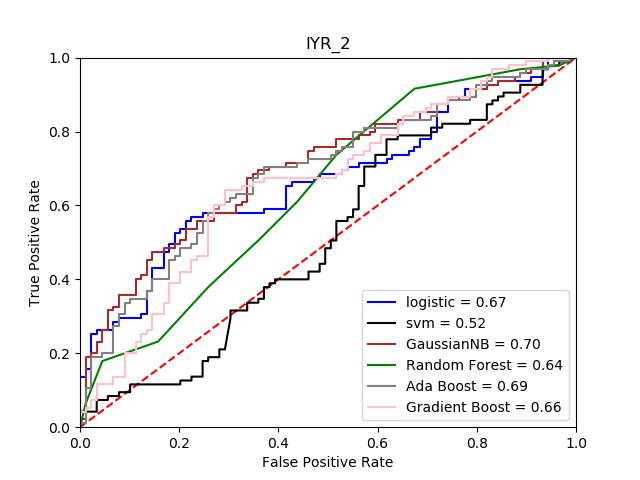
\includegraphics[width=2in]{IYR_2.png}
%\caption{fig2}
\end{minipage}%
}%
\caption{ROC curves related to IYR}
\end{figure}


The accuracy of our machine learning process is below in Table 1.

% Table generated by Excel2LaTeX from sheet 'accuracy_EEM_1'
\begin{table}[h]
  \centering
  \caption{Accuracy}
    \begin{tabular}{clrrrrrrrrrr}
    \toprule
    \textbf{ETF} & \multicolumn{1}{c}{\textbf{Algorithm}} & \multicolumn{5}{c}{\textbf{Y1}}  & \multicolumn{5}{c}{\textbf{Y2}} \\
    \midrule
         &      & \multicolumn{1}{c}{\textbf{TN}} & \multicolumn{1}{c}{\textbf{FP}} & \multicolumn{1}{c}{\textbf{FN}} & \multicolumn{1}{c}{\textbf{TP}} & \multicolumn{1}{c}{\textbf{Accuracy}} & \multicolumn{1}{c}{\textbf{TN}} & \multicolumn{1}{c}{\textbf{FP}} & \multicolumn{1}{c}{\textbf{FN}} & \multicolumn{1}{c}{\textbf{TP}} & \multicolumn{1}{c}{\textbf{Accuracy}} \\
    \midrule
    \multirow{6}[2]{*}{EEM} & Logistic & 95   & 24   & 45   & 20   & 62.50\% & 59   & 31   & 43   & 51   & 59.78\% \\
         & SVM  & 119  & 0    & 65   & 0    & 64.67\% & 79   & 11   & 85   & 9    & 47.83\% \\
         & Naive Bayes & 63   & 56   & 16   & 49   & 60.87\% & 68   & 22   & 46   & 48   & 63.04\% \\
         & Random Forest & 94   & 25   & 43   & 22   & 63.04\% & 64   & 26   & 45   & 49   & 61.41\% \\
         & AdaBoost & 92   & 27   & 35   & 30   & 66.30\% & 64   & 26   & 43   & 51   & 62.50\% \\
         & GradientBoost & 97   & 22   & 37   & 28   & 67.93\% & 56   & 34   & 46   & 48   & 56.52\% \\
    \midrule
    \multirow{6}[2]{*}{EFA} & Logistic & 97   & 19   & 44   & 24   & 65.76\% & 58   & 31   & 49   & 46   & 56.52\% \\
         & SVM  & 114  & 2    & 66   & 2    & 63.04\% & 56   & 33   & 59   & 36   & 50.00\% \\
         & Naive Bayes & 56   & 60   & 9    & 59   & 62.50\% & 73   & 16   & 50   & 45   & 64.13\% \\
         & Random Forest & 94   & 22   & 36   & 32   & 68.48\% & 67   & 22   & 37   & 58   & 67.93\% \\
         & AdaBoost & 91   & 25   & 43   & 25   & 63.04\% & 54   & 35   & 35   & 60   & 61.96\% \\
         & GradientBoost & 89   & 27   & 38   & 30   & 64.67\% & 57   & 32   & 34   & 61   & 64.13\% \\
    \midrule
    \multirow{6}[2]{*}{GLD} & Logistic & 105  & 17   & 38   & 24   & 70.11\% & 69   & 18   & 48   & 49   & 64.13\% \\
         & SVM  & 122  & 0    & 62   & 0    & 66.30\% & 78   & 9    & 84   & 13   & 49.46\% \\
         & Naive Bayes & 66   & 56   & 10   & 52   & 64.13\% & 76   & 11   & 66   & 31   & 58.15\% \\
         & Random Forest & 99   & 23   & 34   & 28   & 69.02\% & 67   & 20   & 42   & 55   & 66.30\% \\
         & AdaBoost & 89   & 33   & 28   & 34   & 66.85\% & 60   & 27   & 38   & 59   & 64.67\% \\
         & GradientBoost & 93   & 29   & 26   & 36   & 70.11\% & 62   & 25   & 37   & 60   & 66.30\% \\
    \midrule
    \multirow{6}[2]{*}{IYR} & Logistic & 95   & 19   & 43   & 27   & 66.30\% & 70   & 19   & 44   & 51   & 65.76\% \\
         & SVM  & 110  & 4    & 70   & 0    & 59.78\% & 59   & 30   & 64   & 31   & 48.91\% \\
         & Naive Bayes & 51   & 63   & 9    & 61   & 60.87\% & 70   & 19   & 46   & 49   & 64.67\% \\
         & Random Forest & 86   & 28   & 42   & 28   & 61.96\% & 57   & 32   & 47   & 48   & 57.07\% \\
         & AdaBoost & 81   & 33   & 39   & 31   & 60.87\% & 58   & 31   & 33   & 62   & 65.22\% \\
         & GradientBoost & 86   & 28   & 41   & 29   & 62.50\% & 63   & 26   & 35   & 60   & 66.85\% \\
    \bottomrule
    \end{tabular}%
  \label{tab:addlabel}%
\end{table}%


\section{Empirical Results}
In this section, we discuss the performance of the portfolios detailed above. Using the weights obtained from the optimization of the above BL models, we calculate buy-and-hold returns on the portfolio for a holding period of one week and repeat the calculation until the end of the sample, and thus obtain the time series of realized portfolio returns. We report the average, standard deviation, skewness and kurtosis of the portfolio returns in the out-of-sample period.

To evaluate the performance of the portfolio, we use the Sharpe ratio and the ratio of reward to down side risk, measured by VaR or CVaR computed from the empirical distribution. As an alternative to Sharpe Ratio we use Omega ratio also referred to as gain-loss ratio. It measures the average gains to average losses in which we define gains as returns above the risk-free rate and losses as returns below the risk-free rate. Hence, investments with a larger Omega measure are preferable. Formally, the omega measure is��

$$\Omega=\dfrac{\dfrac{1}{T}\Sigma^{T}_{t=1}\max{(0,r_{exs,t})}}{\dfrac{1}{T}\Sigma^{T}_{t=1}\max{(0,-r_{exs,t})}}$$

The advantage of the Omega measure is that it does not require any assumption on the distribution of returns. As alternative risk measures besides volatility, we compute the maximum drawdown (MDD). The MDD reflects the maximum accumulated loss that an investor may suffer during the entire investment period if she buys the portfolio at a high price and subsequently sells at the lowest price. We compute MDD of returns as follows:

$$MDD_T=\max_{\tau\in(0,T)}{DD_t}=\max_{\tau\in(0,T)}{\Big(0,\max_{\tau\in(0,\tau)}{(0,r_{\{t,T\}})}\Big)}$$


With these evaluation criteria, we compare the BL portfolios to the market weights portfolio, the naive 1/N portfolio, momentum BL portfolio and mean-variance portfolio.

We initially train logistic regression, support vector machine and naive Bayes classifiers using previous 150 observations and we predict the outcome for 151th observation. Similarly we use the data available till the previous 150 observation to estimate the covariance matrix and using these both estimates we generate the portfolio weights for the 151th day (This is the first day in the cumulative return line). Fixing the initial observation, the estimation sample is then rolled forward by one week; the models are re-estimated and used to generate out-of-sample forecasts for next week, and so on until the end of the sample. We report the rolling window portfolio performance results in the below subsections.

\subsection{Benchmark Portfolios}
We compute two naive diversified portfolios that serve as the benchmark portfolios for the optimization models. First we calculate 1/N strategy which invests equally in the 4 assets. As a second naive diversification strategy we use a weighted portfolio in which each asset obtains the market capitalization weights that is constant over time, which is the neutral point in the Black-Litterman model. Table below shows that while the 1/N portfolio is more diversified, the market weight portfolio performs better. In particular the market weight portfolio generates a $4\%$ higher Sharpe ratio with $13\%$ higher gain-loss ratio.

\subsection{Backtest Performance}
In this section we evaluate the performance of the BL portfolios and classical Mean-Variance portfolio. Momentum BL is based on the belief that the assets�� returns tomorrow are the same as today with $50\%$ confidence level. Machine learning BL is defined in previous sections. Table below suggests that machine learning BL portfolio and Mean-Variance portfolio outperform the 1/N and market portfolio with a huge margin. However, these both portfolios have similar Sharpe ratio, Omega, Reward per unit risk and maximum drawdown when compared to each other .

\begin{table}[h!]
\caption{Result}
\resizebox{\textwidth}{15mm}{
\begin{tabular}{cccccccccc}
\hline
 &Mean & SD p.a & Skewness& Kurtosis & VaR & CVaR & Sharpe Ratio & Omega & MDD\\
\hline
Equal Weighted      & 3.53    & 20.39   &-0.073&14.71&-0.017&-0.221&0.173&0.893&0.752   \\
Marketcapital Weighted  & 2.49    & 18.44   &0.08&12.50&-0.017&-0.190&0.135&0.764&0.650    \\
Momentum BL      & 3.25    & 14.85    &-0.32&10.14&-0.014&-0180&0.219&1.113&0.492  \\
Machine Learning BL      & 28.22    & 18.39    &2.36&27.22&-0.015&-0.038&1.53&12.102&0.138   \\
Mean-Variance & 28.37&18.38 &2.35&27.28&-0.015&-0.037&1.543&12.45&0.138\\
\hline
\end{tabular}}
\label{table:t1}
\end{table}


Figure shows the cumulative return of all the BL portfolios with machine learning derived views as a comparison with the BL portfolio with all the correct views.


\begin{figure*}[!h]
\begin{center}
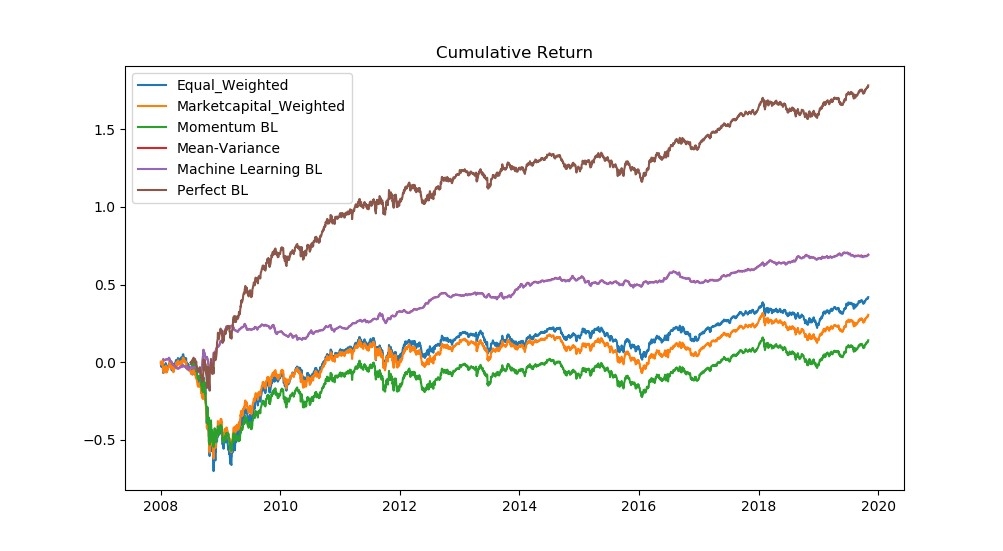
\includegraphics[scale=0.35]{1_6.jpg}
\caption
{Back testing result}
\label{fig:f1}
\end{center}
\end{figure*}




\section{Summary}
It has been shown that BL portfolio isn��t any better than classical Mean-Variance portfolio. This is because the machine learning methods we adopted aren��t effective enough to bring significant outcomes. However, Black-Litterman itself is still a good method for incorporating investor��s view with historical record. When we input correct views in the ��Perfect BL�� model, the result is significantly better. In order to improve machine learning effectiveness, we should be more careful when deciding the view matrix Q and uncertainty matrix ��. Also, restriction on portfolio weights and various optimization methods for constructing a portfolio such minimizing VaR or CVaR can be consider as directions for further study.

\begin{document}
\renewcommand{\bibname}{References}
\begin{thebibliography}{10}
\bibitem{notes} John W. Dower {\emph{Readings compiled for History 21.479.}} 1991.
\bibitem{impj}  The Japan Reader {\emph{Imperial Japan 1800-1945}} 1973: Random House, N.Y.
\end{thebibliography}


\end{document}
